% Notes
% 7.2 Sieve of Eratosthenes needs some citations
%

\documentclass[oneside,12pt]{book}   	% use "amsart" instead of "article" for AMSLaTeX format
\usepackage{savesym}
\usepackage{amsmath}
\usepackage{amssymb}
\usepackage{amsthm}
\usepackage{amsfonts}
\usepackage{epigraph}
\setlength{\epigraphwidth}{4.1in}

\usepackage{color}
\usepackage{makeidx}
\usepackage{microtype}
\usepackage{fancyhdr}
	\fancyhead{}
	\fancyfoot{}
%\renewcommand{\headrulewidth}{0pt}
	\fancyhead[EL, OR]{\thepage}
	\fancyhead[CO]{\rightmark}
	\fancyhead[CE]{\leftmark}
\pagestyle{fancy}

\usepackage[mathscr]{eucal}
\usepackage{setspace}
\usepackage{caption}
\usepackage[pdftex]{graphicx}
\usepackage[perpage,symbol*,norule,multiple,hang,bottom]{footmisc}
\usepackage{pdftricks}
\usepackage[basic,box,gate,oldgate,ic,physics,optics]{circ}
\usepackage{listings}
\usepackage{color}
\usepackage{graphicx}
\usepackage{float}
\usepackage{wrapfig}
\usepackage{ifthen}
\usepackage{courier}
\usepackage[pdftex,bookmarks=true,pdfborder={0 0 0},colorlinks=true,linkcolor=blue,citecolor=blue]{hyperref}
\usepackage[all]{hypcap}
\usepackage{lscape}
\usepackage{tikz}
\usetikzlibrary{matrix,arrows}
\usepackage[h]{esvect}
\usepackage[T1]{fontenc}
\usepackage{frcursive}
\usepackage{polynom}

%\usepackage{tocloft}
%\setlength{\cftchapnumwidth}{2.5em}
%\setlength{\cftsecnumwidth}{2.7em}
%\setlength{\cftsubsecnumwidth}{4.0em}
%\setlength{\cftsubsubsecnumwidth}{4.1em}
%\setlength{\cftparanumwidth}{5 em}
%\setlength{\cftsubparanumwidth}{6 em}

\usepackage{enumitem}
\usepackage{placeins}
\newenvironment{callseries}{\fontfamily{calligra}\selectfont}{}
\newcommand{\textcall}[1]{{\callseries#1}}
\usepackage{fp}
\usepackage{forloop}

\makeindex

\newcounter{ex}
\newcounter{def}
\newcounter{pr}
\newtheorem{axiom}{Axiom}[section]
\newtheorem{problem}{Problem}
\newtheorem{thm}{Theorem}[chapter]
\newtheorem{cor}[thm]{Corollary}
\newtheorem{lem}[thm]{Lemma}
\newtheorem{prop}[thm]{Property}
\newtheorem{proposition}[thm]{Proposition}
\newtheorem{conj}[thm]{Conjecture}
\newtheorem{claim}[thm]{Claim}

\theoremstyle{definition}
\newtheorem{definition}[thm]{Definition}
\newtheorem{algo}[thm]{Alogithm}
\newtheorem{rem}[thm]{Remark}
\newtheorem{exam}[thm]{Example}
\newtheorem{notation}[thm]{Notation}
\newtheorem{idn}[thm]{Identity}


\newcommand{\adj}[1]{\mathrm{adj }~#1}
%\newcommand{\R}[1]{\mathbb{R}^{#1}}
\newcommand{\nul}[1]{\mathrm{nul }~#1}
\newcommand{\col}[1]{\mathrm{col }~#1}
\newcommand{\Span}[1]{\mathrm{Span }\left\{#1\right\}}
\newcommand{\Dim}[1]{\mathrm{dim }~#1}
\newcommand{\Null}[1]{\mathrm{null }~#1}
\newcommand{\Rank}[1]{\mathrm{rank }~#1}
\newcommand{\Range}[1]{\mathrm{range }~#1}
\newcommand{\B}[1]{\textbf{#1}}
\newcommand{\dist}[1]{\mathrm{dist }#1}
\newcommand{\norm}[1]{|\B{#1}|}
\newcommand{\cross}[2]{\vv{#1}\times\vv{#2}}
\newcommand{\dotp}[2]{\vec{#1}\cdot\vec{#2}}

\newcommand{\StirlingTwo}[2]{\genfrac{\{}{\}}{0pt}{}{#1}{#2}}
\newcommand{\StirlingOne}[2]{\genfrac{[}{]}{0pt}{}{#1}{#2}}

\newcommand{\lcm}[1]{\mathrm{lcm }#1}
\newcommand{\p}[2]{\frac{\partial #1}{\partial #2}}
\newcommand{\pp}[2]{\frac{\partial^2 #1}{\partial #2^2}}
\newcommand{\diff}[2]{\frac{d #1}{d #2}}
\newcommand{\Diff}[3]{#1^{(#2)}(#3)}
\newcommand{\del}[0]{\nabla}
\newcommand{\mref}[1]{\ifmathematics \ref{#1} \fi}
\newcommand{\ipv}[2]{\langle\vv{#1},\vv{#2}\rangle}
\newcommand{\ip}[2]{\langle#1,#2\rangle}
\newcommand{\vnorm}[1]{\left|\left|\vv{#1}\right|\right|}
\newcommand{\lnorm}[1]{\left|\left|#1\right|\right|}
\newcommand{\Res}[1]{\mathrm{Res }(#1)}
\newcommand{\Log}[1]{\mathrm{Log }{#1}}

\savesymbol{triangleleft}
\savesymbol{trianglelefteq}
% wide symbols, but mangles triangles. 
\usepackage{mathabx}
\newcommand{\normal}[0]{\triangleleft}
\restoresymbol{ABX}{triangleleft}
\restoresymbol{ABX}{trianglelefteq}

\newcommand{\image}[1]{\mathrm{Im\ }#1}
\newcommand{\vaprhi}[0]{\varphi}
\newcommand{\kernel}[0]{\mathrm{Kern\ }}
\newcommand{\stab}[2]{\mathrm{Stab}_{#1}\left(#2\right)}
\newcommand{\Arg}[0]{\mathrm{Arg\ }}
\newcommand{\orb}[2]{\mathrm{Orb}_{#1}\left(#2\right)}
\newcommand{\aut}[1]{\mathrm{Aut}(#1)}
\newcommand{\inn}[1]{\mathrm{Inn}(#1)}
\newcommand{\syl}[2]{\mathrm{Syl}_{#1}\left(#2\right)}
\newcommand{\set}[1]{\left\{#1\right\}}
\newcommand{\charsg}[0]{\mathrm{\ char\ }}
\newcommand{\card}[1]{\mbox{card }#1}
\newcommand{\seg}[1]{\mbox{seg }#1}

\newcommand{\Lor}[0]{\vee}
\newcommand{\Land}[0]{\wedge}
\newcommand{\disjointunion}[0]{\sqcup}

\newcommand{\floor}[1]{\left\lfloor #1 \right\rfloor}
\newcommand{\ceiling}[1]{\lceil #1 \rceil}

\newcommand{\dom}[0]{\mbox{dom}~}
\newcommand{\ran}[0]{\mbox{ran}~}

\newcommand{\order}[1]{\left| #1 \right|}

\lstset{rangeprefix=\/\/\ ,rangesuffix=\ \/\/}
\lstset{
	xleftmargin=5.0ex,
	firstnumber=1,
	includerangemarker=false,
	numbers=left,
	numberstyle=\tiny,
	language=C,
	frame=single,
	columns=fixed,
	breaklines=true,
	basicstyle=\footnotesize,
	tabsize=4
}

\renewcommand{\footnoterule}{
	\kern -3pt
	\hrule width \textwidth height 0.4pt
	\kern 2.6 pt
}

\title{Project Euler Problems}
\author{Michael E. Conlen}
%\date{}							% Activate to display a given date or no date

\begin{document}
\begin{spacing}{1.618}
\frontmatter
\maketitle

\chapter*{Preface}

Project Euler, \url{http://projecteuler.net/}, is a list of programming problems with a mathematical and algorithmic bent. These problems have solutions that vary from the na\"ive to the sophisticated. While the easiest problems can be effectively solved na\"ively the advanced problems require sophisticated solutions to run effectively. Here we compile a set of solutions in various programming languages along with a mathematical treatment of the sophisticated solutions. Where possible the solutions are generalized for various parameters given in the statement of the problem. 

While Project Euler requests that the solutions not be shared outside of the forums it's clear the solutions are available on the internet. If you have not solved a problem it is up to you to be honest. It is up to  you to realize that understanding the solution is not the point; the point is to have been able to develop the solution yourself. 

\tableofcontents
\lstlistoflistings
\mainmatter

	\chapter{Sum of Natural Numbers Divisible by 3 and 5}
			\begin{quote}
				If we list all the natural numbers below 10 that are multiples of 3 or 5, we get 3, 5, 6 and 9. The sum of these multiples is 23.

				Find the sum of all the multiples of 3 or 5 below 1000.
			\end{quote}

		\section{Introduction}
			
			The na\"ive solutions is to iterate $k$ over the range of integers and if $k\equiv 0\pmod 3$ or $k\equiv 0\pmod 5$ then add the integer to the sum. This solutions is given in Listing \ref{L:1:naive.c}; however this solution runs in $O(n)$ time. A direct computation can be found. 
\lstinputlisting[caption=Problem 1: Na\"ive Solution,label=L:1:naive.c,float=htp]{../src/lang/C/1-1.c}

		\section{Direct Computation}

			Let $n$ be the integer we iterate up through, in this case, $999$\footnote{The problem asks for numbers up to $1000$, thus does not include $1000$ where it is a multiple of $5$.}. Let $m_q=\floor{\frac{n}{q}}$, the number of natural numbers less than $n$ which are multiples of the natural number $q$; then notice that the sum of natural numbers less than $n$ and divisible by $q$ is  
			\begin{alignat}{4}
				q+2q+3q+\dots+m_q q&=q\sum_{k=1}^{m_q}k \notag \\
					&=q\frac{(m_q)(m_q+1)}{2}
			\end{alignat}
			
			If we are summing over the integers which are multiples of $q$ and $r$ then each natural number which is a multiple of both $p$ and $r$ is counted twice; thus we subtract multiples of $qr$; and the solution is 
			\begin{alignat}{4}
				q\frac{(m_q)(m_q+1)}{2}+r\frac{(m_r)(m_r+1)}{2}-qr\frac{(m_{qr})(m_{qr}+1)}{2}
			\end{alignat}
			A generalized version of this program is given in Listing \ref{L:1:1.c}. It's runtime is $O(1)$. 
			\lstinputlisting[caption=Problem 1: C Solution,label=L:1:1.c,float=htp]{../src/lang/C/1-2.c}
			 

	\chapter{Sum of Even Fibonacci Numbers}
		\begin{quote}
			Each new term in the Fibonacci\index{Fibonacci number} sequence is generated by adding the previous two terms. By starting with 1 and 2, the first 10 terms will be:

			\begin{alignat*}{4}
				1, 2, 3, 5, 8, 13, 21, 34, 55, 89, \dots
			\end{alignat*}
			By considering the terms in the Fibonacci sequence whose values do not exceed four million, find the sum of the even-valued terms.
		\end{quote}

		\section{Introduction}
		
			The na\"ive solution is to iterate $k$ over the range of natural numbers computing $F_k$, the $k^{th}$ Fibonacci number, until $F_k>4000000$ and if $F_k$ is even add it to the sum. This solution is given in Listing \ref{L:2:naive.c}. While this solution is generally quick on modern computers it is not efficient. 
			
			\lstinputlisting[caption=Problem 2: Na\"ive Solution,label=L:2:naive.c,float=htp]{../src/lang/C/2-1.c}
		\section{Order of $F_n$}\label{S:2:1}
			We claim that the computation of \texttt{fib(n)} is at least exponential. Let $T(n)$ be the time to compute the $n^{th}$ Fibonacci number and we can see that if we let $T(0)=1$ in units of the time to make the comparison in Line 6, then $T(1)=2 > 1$ and $T(2)=2+T(1)+T(0)> T(1)+T(0)$. In general $T(n)> T(n-1)+T(n-2)$. That is, the estimate is directly related to the Fibonacci numbers themselves.
			
			We may use generating functions\index{generating function}\footnote{See \cite{Wilf2006,GKP94}.} to compute $F_k$. Assume there is a function $f(x)=\sum_{k=0}^\infty F_kx^k$. Recall the defining equation of the Fibonacci numbers;
			\begin{alignat}{4}
				F_{k+2}=F_{k+1}+F_k \label{E:2:1}
			\end{alignat}
			with the boundary conditions $F_0=0$ and $F_1=1$\footnote{This is not precisely the same boundary as $T(0)=1$ and $T(1)=1$; however we can see that it is simply a shift if we consider the negative extension $T(-1)=0$ noting that it preserves the recurrence relation. This preserves the standard numbering of the Fibonacci sequence.}. Multiply equation \ref{E:2:1} by $x^k$,
			\begin{alignat}{4}
				F_{k+2}x^k=F_{k+1}x^k+F_kx^k \label{E:2:2}
			\end{alignat}
			then sum both sides of equation \ref{E:2:2} over all $k$ and compute
			\begin{alignat}{4}
					&&\sum_{k=0}^\infty F_{k+2}x^k&=\sum_{k=0}^\infty F_{k+1}x^k +\sum_{k=0}^\infty F_kx^k \notag \\
				\implies &&\frac{1}{x^2}\sum_{k=0}^\infty F_{k+2}x^{k+2}&=\frac{1}{x}\sum_{k=0}^\infty F_{k+1}x^{k+1} +f(x) \notag \\
				\implies && \frac{1}{x^2}\left(f(x)-F_1x-F_0\right)&=\frac{1}{x}\left(f(x)-F_0\right) + f(x) \notag \\
				\implies && f(x)-F_1x-F_0&=x\left(f(x)-F_0\right)+x^2f(x) \notag \\
				\implies && f(x)-xf(x)-x^2f(x)&=F_1x+F_0-F_0x \notag \\
				\implies && f(x)\left(1-x-x^2\right)&=x \notag \\
				\implies && f(x)&=\frac{x}{1-x-x^2} \label{E:2:3}
			\end{alignat}
			
			If we define $\varphi=\frac{1+\sqrt{5}}{2}$ and $\psi=\frac{1-\sqrt{5}}{2}$ we can see that
			\begin{alignat}{4}
				1-x-x^2=(1-x\varphi)(1-x\psi) \label{E:2:4}
			\end{alignat}
			Thus we can simplify equation \ref{E:2:3} using equation \ref{E:2:4} and partial fraction decomposition
			\begin{alignat}{4}
				\frac{x}{1-x-x^2}&=\frac{x}{(1-x\varphi)(1-x\psi)} \notag \\
					&=\frac{A}{1-x\varphi}+\frac{B}{1+x\psi} \notag \\
					&=\frac{(1-x\psi)A+(1-x\varphi)B}{1-x-x^2} \notag \\
					&=\frac{(A+B)-x(\psi A+\varphi B)}{1-x-x^2} \label{E:2:5}
			\end{alignat}
			and from equation \ref{E:2:5} we can deduce that $A+B=0$ and $\psi A+\varphi B=1$ and compute
			\begin{alignat}{4}
				&&\psi A+\varphi B&=-1 \notag \\
				\implies && \psi A+ \varphi (-A)&=-1 \notag \\
				\implies && (\psi -\varphi) A &=-1 \notag \\
				\implies && A &=\frac{1}{\varphi-\psi} \notag 
			\end{alignat}
			thus
			\begin{alignat}{4}
				B&=-\frac{1}{\varphi-\psi} \notag
			\end{alignat}
			We rewrite equation \ref{E:2:3}
			\begin{alignat}{4}
				\frac{1}{1-x-x^2}&=\frac{1}{\varphi-\psi}\left(\frac{1}{1-x\varphi}-\frac{1}{1-x\psi}\right) \notag \\
					&=\frac{1}{\sqrt{5}}\left(\sum_{k=0}^\infty \varphi^kx^k - \sum_{k=0}^\infty \psi^kx^k\right) \notag \\
					&=\sum_{k=0}^\infty \frac{\varphi^k-\psi^k}{\sqrt{5}} x^k
			\end{alignat}
			thus, recalling that $f(x)=\sum_{k=0}^\infty F_kx^k$ we conclude that
			\begin{alignat}{4}
				F_k=\frac{\varphi^k-\psi^k}{\sqrt{5}} \label{E:2:7}
			\end{alignat}
			
			Since $\order{\psi}<1$ we have that $\psi^k\to 0$ as $k\to\infty$; thus we can see that $F_k$ is exponential in $k$; hence $T(n)$ is at least $O\left(\varphi^n\right)$\footnote{If we work with the estimate that $T_0=1$, $T_1=2$ and $T_{k+2}=T_{k+1}+T_k+m$ where $m$ is the number of operations for the non-recursive steps in the general case, then a similar analysis will show that the runtime is exponential.}. 
		
		\section{Computing \texttt{fib(n)} Directly}
		
			Equation \ref{E:2:7} gives us a closed form for $F_n$ which can be computed for the cost of two calls to \texttt{pow()}. Recall, however, that $\order{\psi}<1$ and, in fact, $\order{\frac{\psi}{\sqrt{5}}}<\frac{1}{2}$; thus we can avoid computation of $\psi^n$ and estimate that $F_k= \frac{\vaprhi^k}{\sqrt{5}}+\epsilon$ and that $\order{\epsilon}<1$; thus we can compute
			\begin{alignat}{4}
				F_k=\floor{\frac{\varphi^k}{\sqrt{5}}+\frac{1}{2}}
			\end{alignat}
			\lstinputlisting[caption=Problem 2: \texttt{fib(n)} Direct,label=L:2:1.c,float=htp]{../src/lang/C/2-2.c}
			This solution is given in Listing \ref{L:2:1.c}. Note that we make use of the fact that for positive numbers typecasting a \texttt{double} to an \texttt{int} type is equivalent to the floor function. In this implementation the runtime of \texttt{fib(n)} is generally $O(1)$ as \texttt{pow()} is implemented in constant time on most processors\footnote{If this is not available exponentiation by squaring is $O(\log n)$.}. This gives the overall program a runtime of $O(\log n)$; but we can do better. 
		
	\section{Sum of Even Fibonacci Numbers}
	
		Notice that the first two Fibonacci numbers are odd, followed by an even. We can see from the defining relation that the even Fibonacci numbers have an index $k\equiv 0\pmod 3$. Moreover, the sum of the even Fibonacci numbers is equal to the sum of the odd Fibonacci numbers before it. We can make use of this fact and the following observation
		\begin{thm}
			Let $F_k$ be the $k^{th}$ Fibonacci number with $F_1=1$ and $F_2=1$; then $\sum_{k=1}^n F_k=F_{n+2}-1$. 
			\begin{proof}[Solution]
				Let $n=1$ then $\sum_{k=1}^1F_k=F_1=1=2-1=F_3-1$; this proves the base case. 
				We compute for arbitrary $n$
				\begin{alignat}{4}
					\sum_{k=1}^nF_k&=F_n + \sum_{k=1}^{n-1}F_k  \notag \\
						&= F_n + F_{n+1} -1 \notag \\
						&= F_{n+2}-1 \notag 
				\end{alignat}
			\end{proof}
		\end{thm}	
		
		Thus, if we know the index of the largest Fibonacci number less than or equal to some value, we can compute the desired sum. 	
			
	\section{Finding the Index}
		
		Notice that if we have a Fibonacci number $F$, then we can compute the index into the sequence, $k$, by 
		\begin{alignat}{4}
			k=\log_\varphi{\left(F\sqrt{5}+\psi^k\right)} \notag
		\end{alignat}
		but without $k$ we must estimate, but $\order{\psi^k}<\frac{1}{2}$ for $k>1$; thus we have that 
		\begin{alignat}{4}
			k<\log_\varphi{\left(F\sqrt{5}+\frac{1}{2}\right)} \notag 
		\end{alignat}
		moreover, the difference is less than $1$ for sufficiently large $F$\footnote{Consider $\frac{d}{dx}\log{(x)}=\frac{1}{x}$.} so let 
		\begin{alignat}{4}
			k=\floor{\log_\varphi{\left(F\sqrt{5}+\frac{1}{2}\right)}} \notag
		\end{alignat}
		
		Now, suppose that $F$ is not a Fibonacci number, but is some natural number; then for some $j\in\mathbb{N}$, $F_j<F<F_{j+1}$ so 
		\begin{alignat}{4}
			j\leq\floor{\log_\varphi{\left(F\sqrt{5}+\frac{1}{2}\right)}}\leq j+1
		\end{alignat}
		thus
		\begin{alignat}{4}
			\floor{\log_\varphi{\left(F\sqrt{5}+\frac{1}{2}\right)}}\in \set{j, j+1}
		\end{alignat}
		We wish to determine $j$, the index of the largest Fibonacci number less than or equal to $F$\footnote{Recall that the problem states \emph{\dots terms in the Fibonacci sequence whose values do not exceed four million\dots}}; so compute $k$ then $F_k$ and if $k=j+1$ $F_k>F$ and if $k=j$ then $F_k\leq F$. In either case we can determine $j$. 
		
		Finally, to get the largest \emph{even} Fibonacci number recall that a Fibonacci number $F_k$ is even if and only if $k\equiv 0\pmod 3$. 

	\section{Direct Computation}

		We combine the results of the last two sections in Listing \ref{L:2:2.c}. 
	
		\lstinputlisting[caption=Problem 2: Direct Solution,label=L:2:2.c,float=htp]{../src/lang/C/2-3.c}

	\section{Generalization}
	
		We generalize the above solution to arbitrary $n$ within the limits of \texttt{unsigned long long} in Listing \ref{L:2:3.c}. 
		
		\lstinputlisting[caption=Problem 2: General Solution,label=L:2:3.c,float=htp]{../src/lang/C/2-4.c}

	\chapter{Largest Prime Factor of $n$}
		\epigraph{The problem of distinguishing prime numbers from composite numbers and of resolving the latter into their prime factors is known to be one of the mots important and useful in arithmetic}{C. F. Gauss}
		\begin{quote}
			The prime factors of 13195 are 5, 7, 13 and 29.

			What is the largest prime\index{prime} factor of the number 600851475143 ?
		\end{quote}
	
		\section{Introduction}
			This algorithm works simply by factoring the integer\footnote{See Appendix \ref{C:Factoring}.} in to prime factors then searching for the largest of the list.  We implement this algorithm in Listing \ref{L:3:naive.c}. 
			
			\lstinputlisting[caption=Problem 3: Na\"ive Solution,label=L:3:naive.c,float=htp]{../src/lang/C/3-1.c}
		
		\section{Prime Factorization}
		
			Factoring the integer into primes is the key component of this algorithm. A simple algorithm is devised which should work well for all but exceedingly large numbers. The header, \texttt{factor.h}, is given in listing \ref{L:factor:factor.h}.  The code in \texttt{factor.c} is given in listing \ref{L:factor:factor.c}. This will be used in several problems. 
		
		\section{\texttt{factorN()}}
		
			The function \texttt{factorN()} works by finding small factors, factoring them out and continuing to look for successively larger factors.
		
			More precisely, let $n\in \mathbb{N}$ be given. Let $n_1=n$. Let $m_2\in\mathbb{N}$ be the largest number such that $2^{m_2}$ divides $n_1$; then set $n_2=\frac{n_1}{2^{m_2}}$. Inductively continue until we have a number $n_k$ such that $k>\sqrt{n_k}$. Since $\set{n_i}$ is a non-decreasing sequence this number $k$ exists. $n_k$ will then be the largest prime factor of $n$. 
			
			Clearly $n_k\mid n$. We can see that $n_k$ is not composite, since if it was the factors of $n_k$ would be smaller than $n_k$ and thus would have been divided out of $n_k$ at the appropriate step in the construction. We are left to show that there is no prime $p$ such that $p>n_k$ and $p\mid n$. This can be seen by looking at the sequence $\set{n_k}$. At each step where $n_k$ is a composite then at least one of it's prime factors is less than $\sqrt{n_k}$; thus, if there are no such prime factors then $n_k$ is prime. 

		\lstinputlisting[caption=\texttt{factor.h},label=L:factor:factor.h,float=htp]{../src/lang/C/factor.h}

		\lstinputlisting[linerange=factorN-end\ factorN,caption=\texttt{factor.c:factorN()},label=L:factor:factor.c,float=htp]{../src/lang/C/factor.c}


	\chapter{Largest Palindrome Product}
	
		\begin{quote}
			A palindromic number reads the same both ways. The largest palindrome made from the product of two 2-digit numbers is $9009 = 91\times 99$.

			Find the largest palindrome made from the product of two 3-digit numbers.
		\end{quote}
		
		\section{Introduction}
	
			This problem presents a few programming issues, the first is to factor an integer and find products of the factors of a given decimal size. The other problem is to be able to represent the sequence of palindrome numbers in a way that we can easily find the predecessor of an element in the sequence.
			
		\section{Palindromic Numbers}
		
			\subsection{Introduction}
				Palindromic numbers\index{palindromic number} are natural numbers which are the same when written (in a given base) forwards and reverse. These numbers can be thought of as having two varieties; those with an odd number of digits and those with an even number of digits.  We can represent a palindromic number by an integer, representing the leading sequence of the integer and a value to indicate whether the number of digits is odd or even; that is, whether the last digit in the integer should be included once or twice respectively. By way of example the palindromic number $10101$ can be represented by $(101, \mathtt{ODD})$ and the number $457754$ can be represented by $(457, \mathtt{EVEN})$. 
		
			\subsection{Predecessor and Successor}	
				To see how to compute predecessor or successor palindromic numbers we consider what the sequence looks like in these terms. The first nine terms are the natural numbers $0$ through $9$. These are represented by the values $(0, \mathtt{ODD})$ through $(9, \mathtt{ODD})$. These numbers are followed by $11, 22, 33, \dots, 99$ which are represented by $(1, \mathtt{EVEN})$ through $(9, \mathtt{EVEN})$. The next portion of the sequence is 
				\begin{alignat*}{4}
					101, 111, 121, 131, \dots, 191, 202, 212, 222, \dots, 292, 303, \dots, 999
				\end{alignat*}
				These are represented by $(10, \mathtt{ODD})$ through $(99, \mathtt{ODD})$. It can be seen that the following portion of the sequence is represented by the values $(10, \mathtt{EVEN})$ through $(99, \mathtt{EVEN})$. 
			
				We can then consider how to compute the successor of a given palindromic number $(a, b)$, written $(a, b)++$. If $a+1\neq 10^k$ for $k\in \mathbb{N}$, $k>0$ then $(a+b)++=(a+1, b)$. That is, $(7, \mathtt{ODD})++=(8, \mathtt{ODD})$ for example. If $a+1=10^k$ for $k\in\mathbb{N}$ and $k>0$ then we have two situations depending on $b$. The successor of $(9, \mathtt{ODD})$ is $(1, \mathtt{EVEN})$, likewise $(99, \mathtt{ODD})++=(10, \mathtt{EVEN})$ and so forth; thus we see that in this case 
				\begin{alignat*}{4}
					(a, b)++=\left(\frac{a+1}{10}, \mathtt{EVEN}\right)
				\end{alignat*}
				In the case where $b=\mathtt{EVEN}$ we have $(a, b)++=(a+1, \mathtt{ODD})$. 
			
				We can write the successor function as 
				\begin{alignat}{4}
					(a, b)++=\left\{\begin{array}{ll}
						(a+1, b),&a+1\neq 10^k,~k\in\mathbb{N},~k>0 \\
						\left(\frac{a+1}{10}, \mathtt{EVEN}\right),&a+1=10^k,~k\in\mathbb{N},~k>0\Land b=\mathtt{ODD} \\
						\left(a+1, \mathtt{ODD}\right),&a+1=10^k,~k\in\mathbb{N},k>0\Land b=\mathtt{EVEN}
					\end{array}\right.
				\end{alignat}
				This function is implemented in \texttt{palindromeSuccessor()} given in Listing \ref{L:palindrome:palindromeSuccessor}. 
				\lstinputlisting[linerange=palindromeSuccessor-end\ palindromeSuccessor,caption=Problem 4: \texttt{palindromeSuccessor()},label=L:palindrome:palindromeSuccessor,float=]{../src/lang/C/palindrome.c}
				
				From the successor we can compute the predecessor function $(a,b)--$, remembering to take care of a  few extra special cases. 
				\begin{alignat}{4}
					(a,b)--=\left\{\begin{array}{ll}
						\mathtt{UNDEFINED},&a=0\Land b=\mathtt{ODD} \\
						\left(a-1, \mathtt{ODD}\right),&a=1\Land b=\mathtt{ODD} \\
						(a-1, b),&a\neq 10^k,k\in\mathbb{N},k>0 \\
						\left(a-1, \mathtt{EVEN}\right),&a=10^k,k\in\mathbb{N},k>0\Land b=\mathtt{ODD} \\
						\left(\left(a-1\right)\cdot 10+9, \mathtt{ODD}\right),&a=10^k,k\in\mathbb{N}\Land b=\mathtt{EVEN}
					\end{array}\right.
				\end{alignat}

				\lstinputlisting[linerange=palindromePredecessor-end\ palindromePredecessor,caption=Problem 4: \texttt{palindromePredecessor()},label=L:palindrome:palindromePredecessor,float=]{../src/lang/C/palindrome.c}

			\subsection{Computing Integer from Representation}
			
				Given the representation of a palindromic number used above we need to compute the actual integer. The value $a$ represents the leading digits which must be shifted some places to the left. The number of places depends on the value of $b$. If $b=\mathtt{ODD}$ then the shift is $\floor{\log_{10}(a)}$. If $b=\mathtt{EVEN}$ then the shift is $\floor{\log_{10}(a)}+1$. 
				
				We might attempt to figure out the value of each place in decimal; but this has been done already by \texttt{sprintf()}. We simply determine the length of $a$, $\mathtt{digits}(a)=\floor{\log_{10}(a)}+1$ to determine the length of the string necessary, $\mathtt{length}(a)+1$, then use \texttt{sprintf()} to place the integer into the string, then treating each character as an integer subtract the value of the string "0" from each value. 
				
				The function \texttt{palindromeInteger()} in Listing \ref{L:palindrome:palindromeInteger} implements this. 
				
				\lstinputlisting[linerange=palindromeInteger-end\ palindromeInteger,caption=Problem 4: \texttt{palindromeInteger()},label=L:palindrome:palindromeInteger,float=]{../src/lang/C/palindrome.c}

			\subsection{Finding an Answer}
			
				Given that we can find the largest palindromic integer less than a given number\footnote{Using the free digits at the start of the integer find the palindromic integer associated with it. Either it satisfies the inequality, at which point any palindromic integer larger than it will not satisfy the inequality, or it's predecessor will satisfy the inequality.} we must determine if it satisfies the condition that it is the product of two integers of a given length. To do this we may start by factoring the integer into a list of $m$ prime factors. Then we can determine if any grouping of the prime factors into to integers will have products of the required length. There are $\sum_{k=0}^m\binom{m}{k}=2^m$ ways to group $m$ prime factors into two groups where we choose $k$ of them for one product and the remaining $m-k$ are in the other product. By enumerating over these $2^m$ groupings we can determine if any grouping satisfies by computation. 
				\lstinputlisting[linerange=twoFactor-end\ twoFactor,caption=Problem 4: \texttt{twoFactor()},label=L:factor:twoFactor,float=htp]{../src/lang/C/factor.c}
				
				This algorithm appears inefficient, possibly even exponential, at first glance; however it should not be too bad. Let $n$ be given. We may write $n=\prod_p p^{k_p}$ where $p$ ranges over all prime numbers and $k_p=0$ if $p\not\mid n$. The number of prime factors $m(n)$ is given by $m(n)=\sum k_p$. We can understand the growth of $m$ by inverting it. The smallest integer which has $x$ prime factors is $2^x$ since any integer which has as many prime factors must have some factor(s) which are not $2$ and all prime numbers not equal to $2$ are greater than $2$. $m\left(2^x\right)=x$; thus the growth of $m$ is $\log_2(n)$; thus an upper bound on the number of groupings we must check for each $n$ is $2^{\log_2(n)}=n$. Summing over all $n$ we have that the algorithm is $O\left(n^2\right)$. 
				
				The function \texttt{twoFactor()} takes a list of (presumably prime) factors and an integer $n$ such that $2^n$ is less than the length of the list and groups the prime factors. The code is given in Listing \ref{L:factor:twoFactor}. 

				In short, the algorithm is as follows
				\begin{enumerate}
					\item	Find largest palindromic number less than $999\times 999$
					\item	For each palindromic number less than $999\times 999$ down to $100\times 100$ do:
						\begin{enumerate}
							\item Factor the palindromic integer
							\item For each grouping of the factors determine if the grouping results in a pair of $3$-digit numbers; if so terminate 
						\end{enumerate}
				\end{enumerate}
				The code for this is given in Listing \ref{L:4-1.c}
				\begin{spacing}{1}
				\lstinputlisting[caption=Problem 4: \texttt{main()},label=L:4-1.c,]{../src/lang/C/4-1.c}
				\end{spacing}
				
	\chapter{Smallest Multiple}
	
		\begin{quote}
			2520 is the smallest number that can be divided by each of the numbers from 1 to 10 without any remainder.

			What is the smallest positive number that is evenly divisible by all of the numbers from 1 to 20?
		\end{quote}
	
		\section{Introduction}
		
			The solution to this problem is the least common multiple\index{least common multiple}\index{lcm|see{least common multiple}} of all integers from $1$ to $20$. 
			\begin{definition}[Least Common Multiple]
				The \emph{least common multiple} of two integers $a$ and $b$ is the smallest $n\in\mathbb{N}$ such that $a\mid n$ and $b\mid n$. We write $\lcm{(a, b)}=n$. 
			\end{definition}
			We can define the $\lcm$ on more than two integers inductively; that is $\lcm{\left(a_0, a_1, \dots, a_n\right)} = \lcm{\left(\lcm{\left(a_0, a_1, \dots, a_{n-1}\right)}, a_n\right)}$. We can compute the $\lcm$ of two integers $a$ and $b$ using the $\gcd$\index{greatest common divisor}\index{gcd|see{greatest common divisor}}. 
			\begin{definition}[Greatest Common Divisor]\index{greatest common divisor}
				For two integers $a$ and $b$ with both not equal to zero the \emph{greatest common divisor} is the $n\in\mathbb{N}$ such that $n\mid a$ and $n\mid b$ and any other number $k\in\mathbb{N}$ which divides both also divides $n$\footnote{This definition could be written more succinctly as the greatest integer which divides both however the definition can be extended to commutative rings where \emph{greatest} fails to have meaning.}. We write $\gcd{(a, b)}=n$. 
			\end{definition}
			
			The connection between the $\lcm$ and the $\gcd$ is
			\begin{alignat}{4}
				\lcm{(a, b)}=\frac{a\cdot b}{\gcd{(a, b)}}\label{E:5:1}
			\end{alignat}
			To prove this we need some lemmas\footnote{See \cite{Mollin2008}}
			\begin{lem}[Euclid's Lemma]\index{Euclid's lemma}\label{Lem:5:1}
				Let $a,b\in\mathbb{Z}\setminus\set{0}$ and $c\in\mathbb{Z}$ such that $c\mid ab$ with $\gcd{(b,c)}=1$ then $c\mid a$. 
				\begin{proof}
					Notice that $\gcd{(ab, ac)}=\order{a}\gcd{(b,c)}=\order{a}$. By hypothesis $c\mid ab$ and clearly $c\mid ac$ so $c\mid\gcd{(ab, ac)}=\order{a}$ that is, $c\mid a$. 
				\end{proof}
			\end{lem}
			
			\begin{lem} \label{Lem:5:3}
				Let $a,b\in\mathbb{N}\setminus\set{0}$, let $\ell =\lcm{(a,b)}$ and $g=\gcd{(a,b)}=1$; then $\ell=ab$. 
				\begin{proof}
					Notice that $b\mid \ell$; thus $b=\ell n$ for some $n\in\mathbb{Z}$. First we show that $a\mid n$ by Lemma \ref{Lem:5:1}. By hypothesis $\gcd{(a,b)}=1$ and by definition $a\mid \ell=bn$ but $a\not\mid b$ so $a\mid n$.
					
					Since $\ell\mid ab$ it follow that $\ell\leq ab$; thus $ab\leq \ell=ab\left(\frac{n}{a}\right)=bn\geq ba$, where we use the fact that $a\mid n\implies n\geq a$. Since $ab\leq \ell \leq ab$ it follows that $\ell=ab$. 			
				\end{proof}
			\end{lem}
			
			\begin{lem} \label{Lem:5:2}
				Let $a,b\in\mathbb{N}\setminus \set{0}$ and let $g=\gcd{(a,b)}$; then $\gcd{\left(\frac{a}{g},\frac{b}{g}\right)}=1$. 
				\begin{proof}
					Let $c\in\mathbb{N}$ such that $c\mid \frac{a}{g}$ and $c\mid \frac{b}{g}$; then $gc\mid a$ and $gc\mid b$. By maximality of $g$ it follows that $c=1$. 
				\end{proof}
			\end{lem}
			\begin{thm}
				Let $a,~b\in\mathbb{Z}\setminus\set{0}$. Let $\ell=\lcm{(a,b)}$ and $g=\gcd{(a,b)}$ then $\ell g=ab$
				\begin{proof}
					 By Lemma \ref{Lem:5:2}, $\gcd{\left(\frac{a}{g},\frac{b}{g}\right)}=1$. By Lemma \ref{Lem:5:3} then $\lcm{\left(\frac{a}{g},\frac{b}{g}\right)}=\frac{ab}{g^2}$; so $ab=g^2\cdot \lcm{\left(\frac{a}{b},\frac{b}{g}\right)}=g\cdot\lcm{(a,b)}=g\ell$ as required. 
				\end{proof}
			\end{thm}
			Thus Equation \ref{E:5:1} is confirmed. This reduces the problem to one of finding the $\gcd$ of two numbers. 
		\section{Computing the Greatest Common Divisor}
		
			Euclidean Division\index{Euclidean division} states that for $a,b\in\mathbb{Z}$ and $b\neq 0$ there exists unique integers $q,~r$ such that $a=bq+r$ and $0\leq r< \order{b}$. We can use this in an algorithm to find $\gcd{(a,b)}$. Let $a$ and $b$ be given; then write 
			\begin{alignat*}{4}
				a&=bq_0+r_0 \\
				b&=r_0q_1+r_1 \\
				r_0&=r_1q_2+r_2 \\
				&\dots \\
				r_{n-2}&=r_{n-1}q_n+r_n
			\end{alignat*}
			By Euclidean Division we can see that the sequence $\set{r_k}$ is decreasing and this procedure terminates when $r_n=0$. We can see then from the equations that $r_{n-1}$ divides $a$ and $b$ by noting that since $r_n=0$ then $r_{n-1}\mid r_{n-1}q_n=r_{n-2}$ and work up the ladder.  Let $c$ be any number that divides $a$ and $b$; then by the first equation $c\mid r_0$, and so forth we see that $c\mid r_k$ for all $k<n$; in particular $c\mid r_{n-1}$; so $c\leq r_{n-1}$ and $r_{n-1}=\gcd{(a,b)}$. This algorithm is implemented in Listing \ref{L:algebra:gcd}. 
			
			\lstinputlisting[linerange=gcd-end\ gcd,caption=Problem 5: \texttt{gcd()},label=L:algebra:gcd,float=]{../src/lang/C/algebra.c}
			
		\section{Solution}
		
			\lstinputlisting[linerange=lcm-end\ lcm,caption=Problem 5: \texttt{lcm()},label=L:algebra:lcm,float=]{../src/lang/C/algebra.c}
			The solution depends on the \texttt{gcd()} function in Listing \ref{L:algebra:gcd}. Additionally we implement the $\lcm$ in Listing \ref{L:algebra:lcm}. We iterate over the integers as shown in \texttt{main()} in Listing 
			
			\lstinputlisting[caption=Problem 5: \texttt{main()},label=L:5-1,float=]{../src/lang/C/5-1.c}
>>>>>>> p5
	
	\chapter{Sum Square Difference}
	
		\begin{quote}
			The sum of the squares of the first ten natural numbers is,
			\begin{alignat*}{4}
				1^2+2^2+\dots +10^2 = 385
			\end{alignat*}
			The square of the sum of the first ten natural numbers is,
			\begin{alignat*}{4}
				\left(1+2+\dots +10\right)^2=3025
			\end{alignat*}
			Hence the difference between the sum of the squares of the first ten natural numbers and the square of the sum is $3025-385=2640$.

			Find the difference between the sum of the squares of the first one hundred natural numbers and the square of the sum. 
		\end{quote}
	
		\section{Introduction}
		
			There is an obvious na\"ive solution which is $O(n)$; however this is unnecessary. We may rewrite the general problem as 
			\begin{alignat}{4}
				\left(\sum_{k=0}^n\right)^2 - \sum_{k=0}^n k^2 \label{E:6:1}
			\end{alignat}
			Both sums in Equation \ref{E:6:1} have closed form solutions. If we happen to have these solutions we may check them by induction; however, we may also derive them using \index{generating function!exponential}\index{exponential generating function}exponential generating functions. 
			
		\section{Exponential Generating Functions}
			Recall the generating functions introduced in Section \ref{S:2:1}. Wilf introduces another form of generating functions in \cite{Wilf2006} called the exponential generating functions. 
			\begin{definition}[Exponential Generating Function]
				Let $\set{a_n}_{n=0}^\infty$ be a sequence; then the \emph{exponential generating function} of $\set{a_n}$ is
				\begin{alignat}{4}
					A(x)=\sum_{n=0}^\infty a_n\frac{x^n}{n!}
				\end{alignat}
			\end{definition}
			The exponential generating function is derived from the sequence $\set{1, 1, 1, \dots}$; that is, $a_n=1$ for all $n$. We can see that in this case $A(x)=e^x$. This leads us to the following theorem
			\begin{thm}\label{T:6:1}
				Let $A(x)$ be the exponential generating function for some sequence $\set{a_n}_{n=0}^\infty$ then the exponential power series for $\set{a_{n+1}}_{n=0}^\infty$ is $A'(x)$. 
				\begin{proof}
					Let $\set{a_n}_{n=0}^\infty$ be a sequence and define $A(x)=\sum_{k=0}^\infty a_k\frac{x^k}{k!}$. We compute
					\begin{alignat}{4}
						A'(x)&=\frac{d}{dx}\sum_{k=0}^\infty a_k\frac{x^k}{k!} \notag \\
							&=\frac{d}{dx}\left[a_0 + \sum_{k=1}^\infty a_k\frac{x^k}{k!}\right] \notag \\
							&=\sum_{k=1}^\infty a_k k \frac{x^{k-1}}{k!} \notag \\
							&=\sum_{k=1}^\infty a_k\frac{x^{k-1}}{(k-1)!} \notag \\
							&=\sum_{k=0}^\infty a_{k+1}\frac{x^k}{k!} \notag 
					\end{alignat}
				\end{proof}
			\end{thm}
			
			With this we can describe the recurrence relationships we work with in terms of differential equations. Recall that for the Fibonacci numbers we had $F_{n+2}=F_{n+1}+F_n$; we can see easily from this that if $f(x)=\sum_{k=0}^\infty F_k \frac{x^k}{k!}$ that $f$ satisfies $f''=f'+f$. Applying the initial conditions that $f(0)=0$ and $f'(0)=1$ we will be rewarded as desired. 
			
		\section{Sum of Integers}\label{S:6:3}
		
			We wish to compute $\sum_{k=0}^\infty k$; thus we write $s_n=\sum_{k=0}^n k$ and note that $s_0=0$ and $s_{n+1}=\sum_{k=0}^{n+1} k = (n+1)+\sum_{k=0}^n k=(n+1)+s_n$. Defining $S(x)=\sum_{n=0}^\infty s_n \frac{x^n}{n!}$ and  using Theorem \ref{T:6:1} we have 
			\begin{alignat}{4}
				S'(x)=S(x)+\sum_{n=0}^\infty (n+1)\frac{x^n}{n!} \label{E:6:2}
			\end{alignat}
	
			We rewrite the last term in Equation \ref{E:6:2} as 
			\begin{alignat}{4}
				\sum_{n=0}^\infty n\frac{x^n}{n!} + \sum_{n=0}^\infty \frac{x^n}{n!}&=e^x + \sum_{n=0}^\infty n\frac{x^n}{n!} \label{E:6:3}
			\end{alignat}
			and we can compute the last term in the right hand side of Equation \ref{E:6:3} as follows\footnote{We could also use the $x\frac{d}{dx}$ operator here and have $\frac{d}{dx}e^x-1=e^x$.}
			\begin{alignat}{4}
				\sum_{n=0}^\infty n\frac{x^n}{n!}&=\sum_{n=1}^\infty n\frac{x^n}{n!} \notag \\
					&=x\sum_{n=1}^\infty n\frac{x^{n-1}}{n!} \notag \\
					&=x\sum_{n=1}^\infty \frac{x^{n-1}}{(n-1)!} \notag \\
					&=x\sum_{n=0}^\infty \frac{x^n}{n!} \notag \\
					&=x e^x
			\end{alignat}
			Thus replacing the last term in Equation \ref{E:6:2} and arranging we have
			\begin{alignat}{4}
				S'(x)-S(x)=(x+1)e^x
			\end{alignat}
			Using the initial condition that $S'(0)=1$ we solve the differential equation\footnote{Everyone always wonders when they will use Calculus if they just want to program.}. Using $D^{-1}$ as the inverse of the differential operator $D=\frac{d}{dx}$ we have 
			\begin{alignat}{4}
				S(x)&=\frac{1}{2}\left(x^2+2x\right)e^x \notag \\
					&=\frac{1}{2}\left(x^2+2x\right)\sum_{n=0}^\infty \frac{x^n}{n!} \notag \\
					&=\frac{1}{2}\left[\sum_{n=0}^\infty \frac{x^{n+2}}{n!} + 2\sum_{n=0}^\infty \frac{x^{n+1}}{n!}\right] \notag \\
					&=\frac{1}{2}\left[D^{-2}\sum_{n=0}^\infty \frac{d^2}{dx^2}\frac{x^{n+2}}{n!} + 2D^{-1}\sum_{n=0}^\infty \frac{d}{dx}\frac{x^{n+1}}{n!}\right] \notag \\
					&=\frac{1}{2}\left[D^{-2}\sum_{n=0}^\infty (n+2)(n+1)\frac{x^n}{n!} + 2D^{-1}\sum_{n=0}^\infty (n+1)\frac{x^n}{n!}\right] \notag
			\end{alignat}
			Now we apply Theorem \ref{T:6:1} in reverse; we can shift the coefficients of the exponential power series to resolve the inverse differential operators and we have
			\begin{alignat}{4}
				S(x)&=\frac{1}{2}\left[\sum_{n=0}^\infty n(n-1)\frac{x^n}{n!} + \sum_{n=0}^\infty 2n\frac{x^n}{n!}\right] \notag \\
					&=\sum_{n=0}^\infty \frac{n(n-1)+2n}{2}\frac{x^n}{n!} \notag \\
					&=\sum_{n=0}^\infty \frac{n(n+1)}{2}\frac{x^n}{n!} \notag 
			\end{alignat}
			thus $s_n=\frac{n(n+1)}{2}$ as we expected\footnote{If we track the constant of integration it becomes part of the $n=0$ term and we can resolve it using the fact that $s_0=0$.}. 
		\section{Sum of Integers Squared}
		
			To compute $\sum_{k=0}^nk^2$ we proceed as we did in the previous section. The differential equation becomes
			\begin{alignat}{4}
				S'-S=\sum_{n=0}^\infty (n+1)^2\frac{x^n}{n!}\label{E:6:4}
			\end{alignat}
			and the last term of Equation \ref{E:6:4} becomes $\left(x^2+3x+1\right)e^x$. The solution to the differential equation is
			\begin{alignat*}{4}
				S(x)=\frac{1}{6}\left(2x^3+9x^2+6x\right)e^x
			\end{alignat*}
			and the coefficients of the exponential power series are computed to 
			\begin{alignat}{4}
				\frac{n(n+1)(2n+1)}{6}
			\end{alignat}
			as expected. 
		\section{Solution}
			Recalling that we were intending to write software we now have all the information for the solution. The difference between the sum of the squares of the first $n$ natural numbers and the square of the sum of the first $n$ natural numbers is 
			\begin{alignat}{4}
				\left(\frac{n(n+1)}{2}\right)^2-\frac{n(n+1)(2n+1)}{6}&=\frac{3n^4+2n^3-3n^2-2n}{12}
			\end{alignat}
			The solution, rather anticlimactically, is given in Listing \ref{L:SSD:SSD}. 
			
			\lstinputlisting[linerange=SSD-end\ SSD,caption=Problem 6: \texttt{SSD()},label=L:SSD:SSD,float=htp]{../src/lang/C/6-1.c}
	
	\chapter{The $n^{th}$ Prime Number}
	
		\begin{quote}
			By listing the first six prime numbers: 2, 3, 5, 7, 11, and 13, we can see that the 6th prime is 13.

			What is the 10 001st prime number?
		\end{quote}
		
		\section{Introduction}
		
			The distribution of primes is known to be irregular. Yitang Zhang has shown that there are infinitely many pairs of consecutive primes such that the difference between them is less than $7\times 10^7$ \cite{Zhang2013}; that is, if $p_k$ is the $k^{th}$ prime number that 
			\begin{alignat}{4}
				\liminf_{n\to\infty}(p_{n+1}-p_n)<7\times 10^7
			\end{alignat}
			
			 Guass conjectured and Hadamard and Poussin later proved a result concerning the prime counting function $\pi(x)$ where $\pi(x)$ is the number of primes less than $x$. The theorem is known as the Prime Number Theorem \cite{Andrews1971}.

			\begin{thm}[Prime Number Theorem]
				\begin{alignat}{4}
					\lim_{x\to\infty}\frac{\pi(x)}{\frac{x}{\log{(x)}}}=1
				\end{alignat} 
			\end{thm}
			If follows from this that 
			\begin{alignat}{4}
				\limsup_{x\to\infty}(p_{n+1}-p_n) = \infty
			\end{alignat}
			since $\frac{\pi(x)}{x}\to 0$ as $x\to \infty$. These results show that finding the $n^{th}$ prime number is difficult. The na\"ive solution would be to check each natural number $k$ in succession testing it for primality by dividing it by every prime found less than $\sqrt{k}$. For small natural numbers, say $n=10001$ this isn't too bad; however for very large natural numbers the divisions becomes expensive\footnote{Multiplication is practically $O(n\log{(n)}\log{(\log{(n)})}$ while addition is $O(\log{(n)})$. }. 
			
		\section{Sieve of Eratosthenes}\index{Sieve of Eratosthenes}\label{S:7:2}
		
			Suppose we wish to determine all the prime numbers less than a given natural number, say $x$. We can list all the natural numbers unto $x$. We know that $2$ is the first prime number so we can remove all multiples of $2$ from the list, that is, $\set{4, 6, 8, \dots}$. The next number remaining is $3$, which we determine to be prime and we remove all multiples of three from the list, $\set{6, 9, 12, \dots}$. We then find $5$ and continue as before. If we have the memory this method works well and only involves addition rather than the more expensive multiplication. The time complexity of the algorithm is $O(n\log{(\log{(n)})})$ at register size and $O(n\log{(n)}\log{(\log{(n)})})$ in bit complexity for large numbers\footnote{Compare to the bit complexity of multiplication.}. The Sieve of Erathothenes is implemented in Listing \ref{L:seive:seiveE}
			
			\lstinputlisting[linerange=sieve-end\ sieve,caption=Problem 7: \texttt{sieveE()},label=L:seive:seiveE,float=htp]{../src/lang/C/sieve.c}
		
		\section{Sizing the Sieve}
			With the Sieve of Eratosthenes we need an estimate of where the $n^{th}$ prime number may be found. While the Prime Number Theorem estimates the density we must be wary to undershooting $x$\footnote{We can imagine techniques which would allow us to extend and continue if we did undershoot these turn out to be unnecessary.}. Before the Prime Number Theorem was proven Chebychev proved a weaker result which provides upper and lower bounds on $\pi(x)$. 
			\begin{thm}[Chebychev's Theorem]\label{T:7:1}
				For $x\geq 8$
				\begin{alignat}{4}
					\frac{\log{(2)}}{4}\cdot \frac{x}{\log{(x)}} \leq \pi(x) \leq 30(\log{(2)})\frac{x}{\log{(x)}}
				\end{alignat}
			\end{thm}
			However, for $n=10001$ these bounds tell us $x\in(3987, 783242)$. More recently Pierre Duscart proves stricter bounds\cite{Duscart1998}. The bounds are
			\begin{alignat}{4}
				\left(1+\frac{1}{\log{(x)}}\right)\frac{x}{\log{(x)}} \leq \pi(x)\leq\left(1+\frac{1.2762}{\log{(x)}}\right)\frac{x}{\log{(x)}} \label{E:7:1}
			\end{alignat}
			where the first bound is valid for $x\geq 599$\footnote{Duscart provides more precise bounds for larger $x$.}. These bounds give an estimate of $x\in(104044, 106571)$. This provides a nice upper bound to work with. 
			
			To generalize this let the number of primes be given, say $n$; then we must solve (simplifying the lower bound in Equation \ref{E:7:1})
			\begin{alignat}{4}
				\frac{x(1+\log{(x)})}{\log{(x)}^2}-n=0
			\end{alignat}
			however this does not succumb to inversion easily. We can however solve this numerically using Newton's method. We compute the derivative
			\begin{alignat}{4}
				\frac{\log{(x)}^2-2}{\log{(x)}^3}
			\end{alignat}
			which gives us the recurrence relationship 
			\begin{alignat}{4}
				x_{n+1}=x_n+\frac{\log{(x_n)}\left(-x_n-x_n\log{(x_n)}+n\log{(x_n)}^2\right)}{-2+\log{(x_n)}^2}
			\end{alignat}
			For an initial $x_n$ we may make use of the Prime Number Theorem and set 
			\begin{alignat}{4}
				x_0&=n\log{(n)}
			\end{alignat}
			\lstinputlisting[linerange=findBound-end\ findBound,caption=Problem 7: \texttt{findBound()},label=L:seive:findBound,float=htp]{../src/lang/C/sieve.c}
			We implement this function in Listing \ref{L:seive:findBound}. Convergence is extremely fast.  
	
	\chapter{Largest Product}
		\begin{quote}
		Find the greatest product of five consecutive digits in the 1000-digit number.

73167176531330624919225119674426574742355349194934 \\
96983520312774506326239578318016984801869478851843 \\
85861560789112949495459501737958331952853208805511 \\
12540698747158523863050715693290963295227443043557 \\
66896648950445244523161731856403098711121722383113 \\
62229893423380308135336276614282806444486645238749 \\ 
30358907296290491560440772390713810515859307960866 \\
70172427121883998797908792274921901699720888093776 \\
65727333001053367881220235421809751254540594752243 \\
52584907711670556013604839586446706324415722155397 \\
53697817977846174064955149290862569321978468622482 \\
83972241375657056057490261407972968652414535100474 \\
82166370484403199890008895243450658541227588666881 \\
16427171479924442928230863465674813919123162824586 \\
17866458359124566529476545682848912883142607690042 \\
24219022671055626321111109370544217506941658960408 \\
07198403850962455444362981230987879927244284909188 \\
84580156166097919133875499200524063689912560717606 \\
05886116467109405077541002256983155200055935729725 \\
71636269561882670428252483600823257530420752963450 \\
		\end{quote} 
	
		\section{Introduction}
		
			There is an obvious na\"ive solution, shown in Listing \ref{L:8:1}. The character string \texttt{string} contains the number string. 
			
			\lstinputlisting[linerange=main-end\ main,caption=Problem 8: \texttt{main()},label=L:8:1,float=htp]{../src/lang/C/8-1.c}

		\section{Other Considerations}
		
			There are two improvements I thought to make to this code. Using a much longer sequence of digits I tested these idea. 
			
			The first idea involves the fact that each digit in the string gets converted from the character to the integer five times. We can convert these once in a single pass before computing products; however this appears to take approximately $26\%$ longer. This solution is given in Listing \ref{L:8:1b}. 
			\lstinputlisting[linerange=main-end\ main,caption=Problem 8: Shifting,label=L:8:1b,float=htp]{../src/lang/C/8-1b.c}

			The second change is that instead of taking $995\times 5$ products I could compute the first product of five digits. For each subsequent product I could divide out the first digit in the current list and multiply the new digit being added to the list. This requires some particular handling of the case where there is a zero in the list, but reduces the number of multiplications by approximately $60\%$. This solution takes approximately twice as long to run. This solution is given in Listing \ref{L:8:2a}. 
			\lstinputlisting[linerange=main-end\ main,caption=Problem 8: Shifting,label=L:8:2a,float=htp]{../src/lang/C/8-2a.c}

	\chapter{Special Pythagorean triplet}
	
		\begin{quote}
			A Pythagorean triplet is a set of three natural numbers, a  b  c, for which,
			\begin{alignat*}{4}
				a^2 + b^2 = c^2
			\end{alignat*}
			For example, $3^2 + 4^2 = 9 + 16 = 2^5 = 52$.

			There exists exactly one Pythagorean triplet for which $a + b + c = 1000$.
			Find the product abc.
		\end{quote}
		
		\section{Introduction}
			The na\"ive solution is to try each combination of $(a, b, c)$ such that $a+b+c=1000$ of which there are $10^6$, determine if they constitute a Pythagorean triplet and compute the product. This solution is given in Listing \ref{L:9:1}. 
			
			\lstinputlisting[linerange=findTriple-end\ findTriple,caption=Problem 9: \texttt{findTriple()},label=L:9:1,float=htp]{../src/lang/C/9-1.c}
			
		\section{Primitive Pythagorean Triplets}
		
			First a definition is in order to be clear,
			\begin{definition}[Pythagorean Triple]\index{Pythagorean triple}
				Let $a,~b,~c\in\mathbb{N}$, then the triple $(a, b, c)$ is a Pythagorean triple if $a^2+b^2=c^2$. 
			\end{definition}
			Thus we could enumerate the pairs of integers $(a,b)$ and see if the resulting $c$ is an integer; however this is slow. There is a special subset of triples that can be used to generate the full set, the primitive triples
			\begin{definition}[Primitive Pythagorean Triple]
				A Pythagorean triple $(a, b, c)$ is said to be  primitive iff $a$, $b$ and $c$ are coprime. 
			\end{definition}
			If $(a,b,c)$ is a primitive Pythagorean triple we can generate any other Pythagorean triple by multiplying by a factor $k$; that is, suppose that $(a,b,c)$ is some non-primitive pythagorean triple, then let $k=\gcd{(a, b, c)}$ and let $a=a'k$, $b=b'k$ and $c=c'k$; then $(a', b', c')$ is a primitive Pythagorean triple since 
			\begin{alignat}{4}
				&&a^2+b^2&=c^2 \notag \\
				\implies && (ka')^2+(kb')^2&=(kc')^2 \notag \\
				\implies && k^2\left(a'^2+b'^2\right)=k^2c' \notag \\
				\implies && a'^2+b'^2=c'^2 \notag 
			\end{alignat}
			and $\gcd{(a', b', c')}=1$. Conversely we can see that taking any primitive triple we can multiply by any $k\in\mathbb{N}$ an the result is still a Pythagorean triple. 
			
			We now show that we can consider any pair of numbers $\gcd{(m,n)}$ such that $m>n$ and $(m,n)=1$ and generate a primitive Pythagorean triple. 
			\begin{thm}
				$(a, b, c)$ is a primitive Pythagorean triple if and only if there exists $m, n\in\mathbb{N}$ such that $m>n$, $\gcd{(m, n)}=1$, $m\not\equiv n\pmod 2$ and $(a, b, c)=\left(2mn, m^2-n^2, m^2+n^2\right)$. 
				\begin{proof}
					Suppose that $m, n\in\mathbb{N}$ with $m>n$ and $\gcd{(m, n)}=1$; then let $a=2mn$, $b=m^2-n^2$ and $c=m^2+n^2$ and we compute
					\begin{alignat*}{4}
						a^2+b^2&=(2mn)^2 + \left(m^2-n^2\right)^2 \\
							&=(2mn)^2 + m^4 -2m^2n^2 + n^4 \\
							&=m^4+2m^2n^2 + n^4  \\
							&=\left(m^2+n^2\right)^2 \\
							&=c^2
					\end{alignat*}
					So that $(a, b, c)$ are a Pythagorean triple. To show that $\gcd{(a, b, c)}=1$ notice that since $m\not\equiv n\pmod{2}$ that $c$ is odd\footnote{WLOG let $m=2k$ be even and $n=2j+1$ be odd; then $c=m^2+n^2=(2k)^2+(2j+1)^2=4k^2+4j^2+4j+1\equiv 1\pmod{2}$.}. Let $p\mid \gcd{(a, b, c)}$, then $p>2$. $p\mid c+b\implies p\mid 2m^2$ and $p\mid c-b\implies p\mid 2n^2$. Since $p$ is odd we have $p\mid \gcd{(m, n)}$ which is a contradiction of $\gcd{(m, n)}=1$; therefore $\gcd{(a, b, c)}=1$ and hence $(a, b, c)$ are primitive.
					
					Conversely suppose that $(a, b, c)$ are a primitive Pythagorean triple so that $a^2+b^2=c^2$. WLOG let $a$ be even. If $b$ is even then so is $c$; but then $2$ divides all three and $(a, b, c)$ is not primitive; so $b$ is odd and hence $c$ is odd; so $b-c$ and $b+c$ are even; set $c-b=2j$ and $c-b=2k$; then 
					\begin{alignat}{4}
						a^2&=c^2-b^2 \notag \\
							&=(c-b)(c+b) \notag 
					\end{alignat} 
					Since $a$ is even we can write 
					\begin{alignat}{4}
						\left(\frac{a}{2}\right)^2&=\left(\frac{(c-b)}{2}\right)\left(\frac{(c+b)}{2}\right)=s\cdot t \notag 
					\end{alignat}
				\end{proof}
			\end{thm}
			We can see that $\gcd{(s, t)}=1$ since $\gcd{(b, c)}=1$\footnote{Suppose $p\mid\gcd{(b,c)}$ then $p\mid b^2$ and $p\mid c^2$ hence $p\mid a^2\implies p\mid a$ which contradicts $\gcd{(a, b, c)}=1$.}. 
			
			Now we show that there exists $m, n\in\mathbb{N}$ such that $s=n^2$ and $t=m^2$.  If $s=1$ or $t=1$ then the claim is vacuously true so we may assume that $s,~t>1$; then consider the prime factorizations as well as that of $\frac{a}{2}$. Since $\gcd{(s, t)}=1$ we can see that each prime factor of $s$ and $t$ must occur twice in $\left(\frac{a}{2}\right)^2$ and hence twice in $s$ and $t$; thus we may set $s=n^2$ and $t=m^2$. Now we can compute
			\begin{alignat}{4}
				c&=t+s&=m^2+n^2 \\
				b&=t-s&=m^2-n^2
			\end{alignat}
			and by extension 
			\begin{alignat}{4}
				x=2mn
			\end{alignat}
			establishing the equality. Suppose that $p\mid \gcd{(m, n)}$ then $p\mid{(b, c)}$ which is a contradiction so $\gcd{(m, n)}=1$, also establishing that $b$ is odd since otherwise $2\mid\gcd{(a, b, c)}$ which is a contradiction. 
			
		\section{Algorithm}

			\lstinputlisting[linerange=findTriple-end\ findTriple,caption=Problem 9: \texttt{findTriple2()},label=L:9:2,float=htp]{../src/lang/C/9-2.c}

			Making use of the established enumeration we may work as follows. For each $m>1$ consider $n<1$ such that $m\not\equiv n\pmod{2}\footnote{For sufficiently large $m$ it will become more efficient to compute the prime factorization of $m$ and enumerate the $n<m$ that are coprime.}$. Construct the triplet $(2mn, m^2-n^2, m^2+n^2)$. If $1000 \equiv 0 \pmod{2m^2+2mn}$ then set
			\begin{alignat}{4}
				k&=\frac{1000}{2m^2+2mn}
			\end{alignat}
			and compute $k^3(2mn)(m^2-n^2)(m^2+n^2)=2k^3\left(m^5n-mn^5\right)$. This solution is given in Listing \ref{L:9:2}. 
				
%			Let $m\in\mathbb{N}$ be given and let $n<m$ with $(m, n)=1$ be given. Let $a=m^2-n^2$ and let $b=2mn$; then $c=m^2+n^2$. Mollin shows that this construction generates a primitive triple and all primitives can be constructed as such\cite{Mollin2008}. Using these facts we can enumerate the set of primitive Pythagorean triples easily and with a third parameter $k$ we can find any triple. 

	\chapter{Summation of Primes}
	
		\begin{quote}
			The sum of the primes below $10$ is $2 + 3 + 5 + 7 = 17$.

			Find the sum of all the primes below two million.
		\end{quote}
		
		\section{Introduction}
			This problem is trivial given the use of the Sieve of Eratosthenes described in Section \ref{S:7:2}. 
			
			\lstinputlisting[linerange=sumPrimes-end\ sumPrimes,caption=Problem 10: \texttt{sumPrimes()},label=L:10:1,float=htp]{../src/lang/C/10-1.c}
	
	\chapter{Largest Product In a Grid}
	
		\begin{quote}
			In the 2020 grid below, four numbers along a diagonal line have been marked in red.

08 02 22 97 38 15 00 40 00 75 04 05 07 78 52 12 50 77 91 08 \\
49 49 99 40 17 81 18 57 60 87 17 40 98 43 69 48 04 56 62 00 \\
81 49 31 73 55 79 14 29 93 71 40 67 53 88 30 03 49 13 36 65 \\
52 70 95 23 04 60 11 42 69 24 68 56 01 32 56 71 37 02 36 91 \\
22 31 16 71 51 67 63 89 41 92 36 54 22 40 40 28 66 33 13 80 \\
24 47 32 60 99 03 45 02 44 75 33 53 78 36 84 20 35 17 12 50 \\
32 98 81 28 64 23 67 10 \textcolor{red}{26} 38 40 67 59 54 70 66 18 38 64 70 \\
67 26 20 68 02 62 12 20 95 \textcolor{red}{63} 94 39 63 08 40 91 66 49 94 21 \\
24 55 58 05 66 73 99 26 97 17 \textcolor{red}{78} 78 96 83 14 88 34 89 63 72 \\
21 36 23 09 75 00 76 44 20 45 35 \textcolor{red}{14} 00 61 33 97 34 31 33 95 \\
78 17 53 28 22 75 31 67 15 94 03 80 04 62 16 14 09 53 56 92 \\
16 39 05 42 96 35 31 47 55 58 88 24 00 17 54 24 36 29 85 57 \\
86 56 00 48 35 71 89 07 05 44 44 37 44 60 21 58 51 54 17 58 \\
19 80 81 68 05 94 47 69 28 73 92 13 86 52 17 77 04 89 55 40 \\
04 52 08 83 97 35 99 16 07 97 57 32 16 26 26 79 33 27 98 66 \\
88 36 68 87 57 62 20 72 03 46 33 67 46 55 12 32 63 93 53 69 \\
04 42 16 73 38 25 39 11 24 94 72 18 08 46 29 32 40 62 76 36 \\
20 69 36 41 72 30 23 88 34 62 99 69 82 67 59 85 74 04 36 16 \\
20 73 35 29 78 31 90 01 74 31 49 71 48 86 81 16 23 57 05 54 \\
01 70 54 71 83 51 54 69 16 92 33 48 61 43 52 01 89 19 67 48 \\
			The product of these numbers is 26  63  78  14 = 1788696.

			What is the greatest product of four adjacent numbers in the same direction (up, down, left, right, or diagonally) in the 2020 grid?
		\end{quote}
		
		\section{Introduction}
			This is easily solved by searching through all the possible products as shown in Listing \ref{L:11:1}. Note that \texttt{grid} is defined to be a two dimensional array containing the grid of numbers. 
			
			\lstinputlisting[linerange=findMax-end\ findMax,caption=Problem 11: \texttt{findMax()},label=L:11:1,float=htp]{../src/lang/C/11-1.c}
	
	\chapter{Highly divisible triangular number}
	
		\begin{quote}
			The sequence of triangle numbers is generated by adding the natural numbers. So the 7th triangle number would be 1 + 2 + 3 + 4 + 5 + 6 + 7 = 28. The first ten terms would be:
			\begin{alignat*}{4}
				1, 3, 6, 10, 15, 21, 28, 36, 45, 55, \dots
			\end{alignat*}
			Let us list the factors of the first seven triangle numbers:
			\begin{alignat*}{4}
				 1&: 1\\
				 3&: 1,3\\
				 6&: 1,2,3,6\\
				10&: 1,2,5,10\\
				15&: 1,3,5,15\\
				21&: 1,3,7,21\\
				28&: 1,2,4,7,14,28\\
			\end{alignat*}
			We can see that 28 is the first triangle number to have over five divisors.

			What is the value of the first triangle number to have over five hundred divisors?
		\end{quote}
		
		\section{Introduction}
		
			The triangle numbers are the natural numbers of the form $\sum_{k=1}^n k=\frac{n(n+1)}{2}$ as noted in Section \ref{S:6:3}. To count the divisors of a number $x$ we write $x=\prod_{j=1}^r{p_j^{\alpha_j}}$ then for each $j$ tuple $(\alpha_1, \alpha_2, \dots, \alpha_r)$ there is a unique divisor; hence the number of divisors is $\prod_{j=1}^r(\alpha_j+1)$. 
			
			The solution in Listing \ref{L:12:1} simply enumerates the triangle numbers factoring each integer and scans the list of prime factors for the largest, denoted \texttt{maxPrime}. The algorithm then allocates an array, \texttt{factorList} of length \texttt{maxPrime +1} which is zero filled. This allows us to scan the list of prime factors and increment the element \texttt{factorList[list[j]]} to count the exponent of each prime number. 
			
			We could scan the entire list taking the product of each element \texttt{+1}; however this is likely inefficient, instead we scan the prime factor list for indexes into \texttt{factorList} and add the appropriate value to the product; then set the value to zero so that factors of multiplicity greater than $1$ are not counted multiple times. 

			\lstinputlisting[linerange=findTriangle-end\ findTriangle,caption=Problem 12: \texttt{findTriangle()},label=L:12:1,float=htp]{../src/lang/C/12-1.c}
	
	\chapter{Large Sum}
		\begin{quote}
			Work out the first ten digits of the sum of the following one-hundred 50-digit numbers. \dots
		\end{quote}
		The number is listed in Appendix \ref{A:P:13}. 
		
		\section{Introduction}
		
			We could use several \texttt{uint64\_t} integers to break the $50$ digit number into three $19$ digit components then write our own addition function; however the GNU Multiple Precision library handles this type of problem excellently at which point the problem becomes trivial, as in Listing \ref{L:13:1}. 
			
			\lstinputlisting[linerange=findSum-end\ findSum,caption=Problem 13: \texttt{findSum()},label=L:13:1,float=htp]{../src/lang/C/13-1.c}
	
	\chapter{Largest Collatz Sequence}
		\begin{quote}
			The following iterative sequence is defined for the set of positive integers:
			\begin{alignat*}{4}
				n&\to  \frac{n}{2}&\hspace{1 cm}\textrm{(n is even)} \\
				n&\to  3n + 1&\hspace{1 cm} \textrm{(n is odd)}
			\end{alignat*}

			Using the rule above and starting with 13, we generate the following sequence:
			\begin{alignat*}{4}
				13 \to 40 \to 20 \to 10 \to 5 \to 16 \to 8 \to 4 \to 2 \to 1
			\end{alignat*}
			It can be seen that this sequence (starting at 13 and finishing at 1) contains 10 terms. Although it has not been proved yet (Collatz Problem), it is thought that all starting numbers finish at 1.

			Which starting number, under one million, produces the longest chain?

			NOTE: Once the chain starts the terms are allowed to go above one million.
		\end{quote}
		
	\section{Introduction}
	
		There is a simple na\"ive solution of iterating over each value and computing the chain. This solution is given in Listing \ref{L:14:1}. Running this algorithm though we can see that for the relatively small input of $10^6$ that this algorithm takes $0.270~s$; moreover the algorithm appears to be super-linear in time.  

		\lstinputlisting[linerange=findMaxChain-end\ findMaxChain,caption=Problem 14: \texttt{findMaxChain()},label=L:14:1,float=htp]{../src/lang/C/14-1.c}
	
	\section{Memoization}
		Suppose we compute the chain 
		\begin{alignat*}{4}
			13 \to 40 \to 20 \to 10 \to 5 \to 16 \to 8 \to 4 \to 2 \to 1
		\end{alignat*}
		We could save these results noting that $2$ generates  a chain of length 2, $4$ generates a chain of length $3$ and s forth. Then, next time a chain hits one of these values we no longer need to compute the rest of the chain. The primary issue with using memoization in this algorithm is that it's impossible to tell the maximum value one might encounter. In the above sequence the initial value of $30$ reaches a maximum of $40$. With this in mind we identify a maximum size of our memoization table and allocate memory for that table alone. While chains which have large numbers may not make complete use of the table the performance gains are still substantial. 
		
		The algorithm consists of two parts. The first is to compute the chain, storing the chain in the array \texttt{z[]}, until we reach a point in the table \texttt{memo[]}. Notice that the array \texttt{z[]} is used as a queue and is dynamically extended as necessary by factors of $2$. The second part then stores values in the chain which fall within the limits of \texttt{memo[]} in the table for later use. While the algorithm, given in Listing \ref{L:14:2}, is considerably more complex it is an order of magnitude faster for inputs which generate chains with values about to the limits of \texttt{uint64\_t}. 
		\clearpage
		\begin{spacing}{1}
			\lstinputlisting[linerange=findMaxChain-end\ findMaxChain,caption=Problem 14 Memoized: \texttt{findMaxChain()},label=L:14:2]{../src/lang/C/14-2.c}
		\end{spacing}		
		\clearpage
	
	\chapter{Lattice Paths}
		\begin{quote}
			Starting in the top left corner of a 22 grid, and only being able to move to the right and down, there are exactly 6 routes to the bottom right corner as in Figure \ref{Fig:15:1}\footnote{From the project Euler website \url{http://projecteuler.net/problem=15}.}. How many such routes are there through a $20\times 20$ grid?
			\begin{figure}
				\centering
					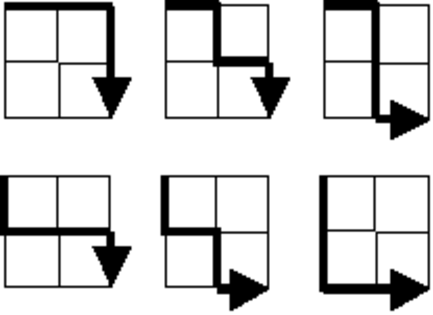
\includegraphics[]{p_015.pdf}
				\caption{Paths through $2\times 2$ Grid}\label{Fig:15:1}
			\end{figure}
		\end{quote}
		\section{Introduction}
		
			We can consider the possible paths through the grid as a sequence of movements right and movements down\footnote{We assume that we are never moving away from the destination, otherwise the number of paths are infinite.}. If we identify these with zero and one respectively we can write a path as a binary number. The length of the binary number is the taxicab distance\index{taxicab distance}\footnote{The taxicab distance, also known as the Manhattan distance or the $L_1$ norm\index{norm} in two dimensions for two points $x=(x_1, x_2)$ and $y=(y_1, y_2)$ is $d(x, y)=\sum_{k=1}^2\order{x_k-y_k}$.} from the upper left corner to the lower right corner. For grid of size $m\times n$ the distance is $m+n$. 
			
			Considering that we must move exactly $m$ to the left and exactly $n$ down we can see that the representation must have exactly $m$ zeros and $n$ ones. We can solve this problem by counting. If we write down where each zero is located there are $(m+n)$ options for the first zero, $(m+n-1)$ for the second and so forth down to $(n)$. For example in a $3x3 grid$ we have six movements, we might places the zeroes in the first, second and fifth location, say $(1, 2, 5)$, but we might also identify $(1, 5, 2)$, $(2, 5, 1)$ and so forth. We must divide by the permutations of $m$ objects, that is $m!$; thus the solution is 
			\begin{alignat}{4}
				\frac{(m+n)!}{m!n!}
			\end{alignat}
		
		\section{Programming the Solution}
		
			While we can write down the solution as 
			\begin{alignat}{4}
				\frac{40!}{20!20!}
			\end{alignat}
			we are asked to encode the solution. Notice that $\log_2{(40!)}=159.159$. Clearly until we have $256$ bit numbers the computation is not straight forward; thus we are forced to use GMP (or similar). The solution is given in Listing \ref{L:15:1}. 
			
			\lstinputlisting[linerange=findPaths-end\ findPaths,caption=Problem 15: \texttt{findPaths()},label=L:15:1,float=]{../src/lang/C/15-1.c}
			
	\chapter{Power digit sum}
		\begin{quote}
			$2^{15}=32768$ and the sum of it's digits is $3+2+7+6+8=26$. 
			
			What is the sum of the digits of the number $6^{1000}$?
		\end{quote}
		\section{Introduction}
		
			This is another problem which becomes trivial once GMP is employed. We need only use GMP to write the number as a string using \texttt{mpz\_get\_str()}. The length of the string can be computed using \texttt{mpz\_sizeinbase()}. The solution is give in Listing \ref{L:16:1}
			
			\lstinputlisting[linerange=findSum-end\ findSum,caption=Problem 16: \texttt{findSum()},label=L:16:1,float=]{../src/lang/C/16-1.c}
			
		
	
\appendix

	\chapter{Problem 13}\label{A:P:13}
	
		\begin{quote}
37107287533902102798797998220837590246510135740250 \\
46376937677490009712648124896970078050417018260538 \\
74324986199524741059474233309513058123726617309629 \\
91942213363574161572522430563301811072406154908250 \\
23067588207539346171171980310421047513778063246676 \\
89261670696623633820136378418383684178734361726757 \\
28112879812849979408065481931592621691275889832738 \\
44274228917432520321923589422876796487670272189318 \\
47451445736001306439091167216856844588711603153276 \\
70386486105843025439939619828917593665686757934951 \\
62176457141856560629502157223196586755079324193331 \\
64906352462741904929101432445813822663347944758178 \\
92575867718337217661963751590579239728245598838407 \\
58203565325359399008402633568948830189458628227828 \\
80181199384826282014278194139940567587151170094390 \\
35398664372827112653829987240784473053190104293586 \\
86515506006295864861532075273371959191420517255829 \\
71693888707715466499115593487603532921714970056938 \\
54370070576826684624621495650076471787294438377604 \\
53282654108756828443191190634694037855217779295145 \\
36123272525000296071075082563815656710885258350721 \\
45876576172410976447339110607218265236877223636045 \\
17423706905851860660448207621209813287860733969412 \\
81142660418086830619328460811191061556940512689692 \\
51934325451728388641918047049293215058642563049483 \\
62467221648435076201727918039944693004732956340691 \\
15732444386908125794514089057706229429197107928209 \\
55037687525678773091862540744969844508330393682126 \\
18336384825330154686196124348767681297534375946515 \\
80386287592878490201521685554828717201219257766954 \\
78182833757993103614740356856449095527097864797581 \\
16726320100436897842553539920931837441497806860984 \\
48403098129077791799088218795327364475675590848030 \\
87086987551392711854517078544161852424320693150332 \\
59959406895756536782107074926966537676326235447210 \\
69793950679652694742597709739166693763042633987085 \\
41052684708299085211399427365734116182760315001271 \\
65378607361501080857009149939512557028198746004375 \\
35829035317434717326932123578154982629742552737307 \\
94953759765105305946966067683156574377167401875275 \\
88902802571733229619176668713819931811048770190271 \\
25267680276078003013678680992525463401061632866526 \\
36270218540497705585629946580636237993140746255962 \\
24074486908231174977792365466257246923322810917141 \\
91430288197103288597806669760892938638285025333403 \\
34413065578016127815921815005561868836468420090470 \\
23053081172816430487623791969842487255036638784583 \\
11487696932154902810424020138335124462181441773470 \\
63783299490636259666498587618221225225512486764533 \\
67720186971698544312419572409913959008952310058822 \\
95548255300263520781532296796249481641953868218774 \\
76085327132285723110424803456124867697064507995236 \\
37774242535411291684276865538926205024910326572967 \\
23701913275725675285653248258265463092207058596522 \\
29798860272258331913126375147341994889534765745501 \\
18495701454879288984856827726077713721403798879715 \\
38298203783031473527721580348144513491373226651381 \\
34829543829199918180278916522431027392251122869539 \\
40957953066405232632538044100059654939159879593635 \\
29746152185502371307642255121183693803580388584903 \\
41698116222072977186158236678424689157993532961922 \\
62467957194401269043877107275048102390895523597457 \\
23189706772547915061505504953922979530901129967519 \\
86188088225875314529584099251203829009407770775672 \\
11306739708304724483816533873502340845647058077308 \\
82959174767140363198008187129011875491310547126581 \\
97623331044818386269515456334926366572897563400500 \\
42846280183517070527831839425882145521227251250327 \\
55121603546981200581762165212827652751691296897789 \\
32238195734329339946437501907836945765883352399886 \\
75506164965184775180738168837861091527357929701337 \\
62177842752192623401942399639168044983993173312731 \\
32924185707147349566916674687634660915035914677504 \\
99518671430235219628894890102423325116913619626622 \\
73267460800591547471830798392868535206946944540724 \\
76841822524674417161514036427982273348055556214818 \\
97142617910342598647204516893989422179826088076852 \\
87783646182799346313767754307809363333018982642090 \\
10848802521674670883215120185883543223812876952786 \\
71329612474782464538636993009049310363619763878039 \\
62184073572399794223406235393808339651327408011116 \\
66627891981488087797941876876144230030984490851411 \\
60661826293682836764744779239180335110989069790714 \\
85786944089552990653640447425576083659976645795096 \\
66024396409905389607120198219976047599490197230297 \\
64913982680032973156037120041377903785566085089252 \\
16730939319872750275468906903707539413042652315011 \\
94809377245048795150954100921645863754710598436791 \\
78639167021187492431995700641917969777599028300699 \\
15368713711936614952811305876380278410754449733078 \\
40789923115535562561142322423255033685442488917353 \\
44889911501440648020369068063960672322193204149535 \\
41503128880339536053299340368006977710650566631954 \\
81234880673210146739058568557934581403627822703280 \\
82616570773948327592232845941706525094512325230608 \\
22918802058777319719839450180888072429661980811197 \\
77158542502016545090413245809786882778948721859617 \\
72107838435069186155435662884062257473692284509516 \\
20849603980134001723930671666823555245252804609722 \\
53503534226472524250874054075591789781264330331690 
		\end{quote}
	
		
	\bibliography{Euler}
	\bibliographystyle{ieeetr}	
	\printindex
\end{spacing}
\end{document}  
